% Same Model, Different Service -- Anonymous Submission
\documentclass[11pt]{article}
\usepackage{acl}
\usepackage{times}
\usepackage{latexsym}
\usepackage[T1]{fontenc}
\usepackage[utf8]{inputenc}
\usepackage{microtype}
\usepackage{amsmath}
\usepackage{booktabs}
\usepackage{multirow}
\usepackage{xspace}
\usepackage{url}
\usepackage{tikz}
\usetikzlibrary{arrows.meta,positioning,shapes.geometric,calc}
\usepackage{pgfplots}
\pgfplotsset{compat=1.18}
\usepackage{setspace}
\usepackage{mdframed}
\usepackage{enumitem}

\title{Same Model, Different Service: Detecting Provider-Induced\\
Reliability Failures in API-Based LLM Evaluation}

\author{Anonymous ACL submission}

\begin{document}
\maketitle
\raggedbottom
\setlength{\dbltextfloatsep}{5pt plus 1pt minus 1pt}
\setlength{\textfloatsep}{5pt plus 1pt minus 1pt}
\setlength{\floatsep}{3pt plus 1pt minus 1pt}
\setlength{\abovedisplayskip}{4pt plus 1pt minus 1pt}
\setlength{\belowdisplayskip}{4pt plus 1pt minus 1pt}
\setlength{\abovedisplayshortskip}{2pt plus 1pt minus 1pt}
\setlength{\belowdisplayshortskip}{2pt plus 1pt minus 1pt}
\setlength{\abovecaptionskip}{4pt plus 1pt minus 1pt}
\setlength{\belowcaptionskip}{2pt plus 1pt minus 1pt}

%-------------------------------------------------------------------
\begin{abstract}
Researchers increasingly evaluate open-weight language models through
API aggregators that route a single model name to many third-party
providers, each serving the same weights under different
infrastructure, quantization, and configuration. We ask whether this
invisible routing threatens the validity of API-based evaluation, and
introduce a pre-registered harness that separates two properties prior
work has conflated: whether a provider returns a correct answer, and
whether it returns a complete one. Across two open models (12 and 6
live providers respectively) and three benchmarks (GSM8K, MMLU,
HumanEval), we find clean-completion accuracy is provider-invariant:
no provider pair shows a statistically separated gap under our
pre-registered threshold. Reliability is not. One provider
(anonymized as Provider~C for review) shows a serving-level truncation
pathology absent from every other provider we test, recurring across
two benchmarks and both models we evaluate it on (16.2\% and 20\%
truncation rates, independently replicated), and manifesting as both
overt failures (\texttt{finish\_reason=error}) and silently mislabeled
ones (\texttt{finish\_reason=stop} on incomplete output). The
pathology is not explained by output length (Spearman
$\rho{=}{-}0.10$) but is deterministic and item-specific: at
temperature 0, a fixed subset of GSM8K items accounts for the large
majority of truncations, with 31 of 300 items failing on all three
repeated trials against fewer than one expected by chance. We formalize
this with a Failure Consistency Coefficient, an intraclass correlation
statistic that confirms high item-level determinism (0.70--0.94) across
three benchmark-model cells while remaining undefined, as it should,
for every clean peer provider. We further show that every silent-truncation candidate our own detector flagged
on a second model was, on manual audit, a complete and correct answer
misclassified by a formatting heuristic, underscoring that neither
provider self-reports nor naive completeness checks can be trusted
without content-level verification. A systematic survey of eight
candidate open models for multi-provider coverage finds only two with
sufficient breadth for this kind of study, itself evidence that wide
multi-provider serving concentrates on a small number of popular
models. We release our harness, a reporting checklist for API-based
evaluation, and all raw per-call logs with checksums (link in the
Ethics Statement).
\end{abstract}

%-------------------------------------------------------------------
\section{Introduction}

A benchmark score reported for an open-weight model such as
Llama-3.3-70B is often treated as a property of the model. In
practice, when that model is accessed through an API aggregator such
as OpenRouter, the score is a property of the model, the serving
provider, the disclosed or undisclosed quantization, and the date the
call was made. Aggregators route a single model identifier across many
third-party providers, and those providers differ in hardware,
precision, batching policy, and software stack. A recent practitioner
account of this problem is blunt about the consequence: an evaluation
suite that checked only the model card missed that a provider was
serving a quantized variant on a different kernel with non-default
sampling parameters, and the regression went unnoticed until it showed
up in production behavior \citep{same_model_service2026}.

Two questions follow from this. First, does provider routing change
what a benchmark measures: does accuracy actually vary across
providers serving the same weights, enough to change which model looks
better. Second, and less studied, does provider routing change whether
a benchmark measurement is trustworthy at all: can a provider fail to
complete a generation in a way that a standard accuracy harness
silently records as a wrong answer rather than a missing one. We treat
these as two distinct axes, accuracy and reliability, and build a
pre-registered measurement protocol that reports both.

We find that the first axis is close to a non-issue for the models and
benchmarks we test: accuracy is provider-invariant within our
pre-registered threshold, and our own initial data made a compelling
case for provider-driven accuracy variance until we discovered that
the apparent effect was a truncation artifact, not a real difference.
The second axis is the opposite story. One provider in our set
exhibits a truncation pathology that no other provider shows, replicated
independently at two different sample sizes, appearing in two different
forms depending on the model, and traceable to specific input items
rather than to random infrastructure noise.

Our contributions are:

\begin{itemize}[itemsep=2pt, topsep=3pt, parsep=1pt]
\item \textbf{A two-axis measurement protocol.} We separate answer
  correctness from generation completeness, with a pre-registered
  taxonomy of failure types (overt error, silently mislabeled, and
  our own token-budget artifact) and an audit step that verifies every
  automatically flagged failure against the raw completion text before
  it is counted.

\item \textbf{An audited empirical result.} Across three benchmarks and
  two models, clean-completion accuracy is provider-invariant. One
  provider shows a real, replicated, content-triggered reliability
  failure that we rule out as a length effect and localize to a
  reproducible subset of inputs, which we quantify with a Failure
  Consistency Coefficient, an intraclass-correlation statistic that
  is undefined for every clean peer and 0.70--0.94 for the affected
  provider across three benchmark-model cells.

\item \textbf{A demonstrated need for the audit step.} We report two
  cases, on two different benchmarks, where an automated failure
  detector produced false positives that a naive study would have
  reported as findings. Both were complete, correct answers that used
  a non-standard closing phrase instead of the expected delimiter.

\item \textbf{A public harness and reporting checklist.} We release
  the measurement harness, frozen benchmark item sets, provider
  snapshots, and checksummed raw logs for all reported cells, together
  with a short checklist for reporting API-based evaluation results.
\end{itemize}

%-------------------------------------------------------------------
\section{Related Work}

\textbf{Operational variation across providers.} Concurrent work
studies the same model served by different providers as distinct
service objects, comparing price, latency, context length, and
protocol behavior \citep{same_model_service2026}. That work explicitly
treats its cross-provider comparisons as weaker than a controlled
experiment and does not test semantic quality or accuracy equivalence.
We measure exactly the dimension left open: whether provider choice
changes what a benchmark reports, and whether a provider can fail in a
way that a standard harness would silently misgrade.

\textbf{Output consistency across providers.} A related line of work
measures cross-provider output consistency in a finance setting, using
identity and drift metrics on repeated calls and finding that some
models stay perfectly consistent across deployments while others show
severe run-to-run drift \citep{output_drift2025}. That work is scoped
to a single domain and measures whether outputs match each other, not
whether a generation completed or whether the reported answer is
correct. We measure benchmark accuracy and a distinct notion of
generation completeness across general reasoning, knowledge, and code
benchmarks.

\textbf{Quantization and accuracy.} A body of work establishes that
reduced-precision serving can degrade accuracy under controlled
conditions \citep{quantization_accuracy2025}. Our contribution is not
this mechanism, which we do not dispute, but an in-the-wild
demonstration that once quantization and configuration are hidden
behind a single model name on a real aggregator, the accuracy effect
we actually observe is negligible, while an unrelated reliability
effect is not. We explicitly test and reject an output-length
explanation for our reliability finding, which rules out the simplest
version of a quantization-driven capacity story.

\textbf{Determinism at temperature zero.} Recent systems work shows
that temperature-zero inference is not bit-identical across repeated
calls because of batch-size-dependent reduction kernels, and provides
batch-invariant kernels that restore exact reproducibility at a
throughput cost \citep{thinking_machines2025}. That line of work is
about output-level nondeterminism: the same prompt can produce
different tokens on different calls. Our finding is the reverse
pattern at the level of failures: a specific provider fails on the
same items every time at temperature zero, which is evidence of a
deterministic, content-triggered defect rather than the kind of
random batch-composition noise that motivates batch-invariant
kernels.

\textbf{Benchmark auditing.} Work on contamination detection has shown
that popular auditing methods themselves fail under distribution shift
and at benchmark scale \citep{reliability_gap_audit2026}. We view our
audit step in the same spirit: an automated flag is a candidate, not a
finding, and we show concretely what happens when that principle is
skipped.

%-------------------------------------------------------------------
\section{Method}

Figure~\ref{fig:harness} shows the full measurement pipeline. Every
call is pinned to a specific provider, verified on return, and routed
into one of four outcome classes before any accuracy number is
computed. Silent-failure candidates are never counted directly; they
pass through a manual audit step first.

\begin{figure*}[t]
\centering
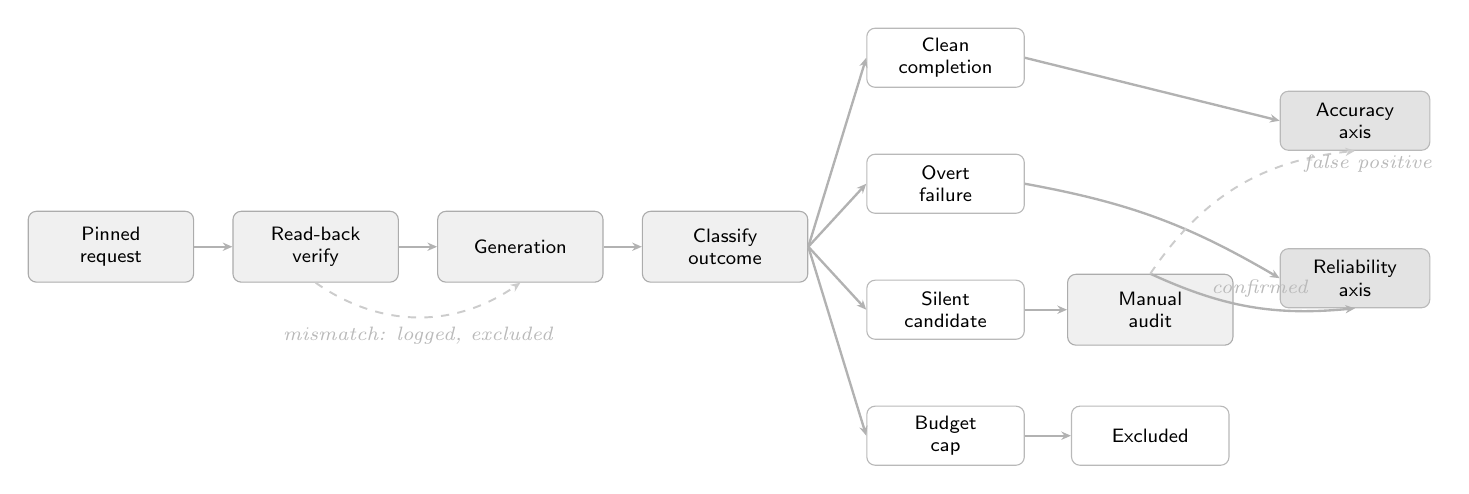
\begin{tikzpicture}[every node/.style={font=\scriptsize\sffamily},
  stagebox/.style={draw=gray!65, fill=gray!12, rounded corners=3pt,
              align=center, minimum width=2.1cm, minimum height=0.9cm,
              inner sep=2pt},
  leafbox/.style={draw=gray!55, fill=white, rounded corners=3pt,
              align=center, minimum width=2.0cm, minimum height=0.75cm,
              inner sep=2pt},
  axisbox/.style={draw=gray!55, fill=gray!22, rounded corners=3pt,
              align=center, minimum width=1.9cm, minimum height=0.75cm,
              inner sep=2pt},
  arr/.style={-{Stealth[length=3.5pt,width=3pt]}, gray!60, line width=0.85pt},
  darr/.style={-{Stealth[length=3.5pt,width=3pt]}, gray!40, dashed,
               line width=0.7pt},
  lbl/.style={font=\scriptsize\itshape, text=gray!55},
]

% main pipeline, left to right
\node[stagebox]                        (req) at (0,0)   {Pinned\\request};
\node[stagebox]                        (rb)  at (2.6,0) {Read-back\\verify};
\node[stagebox]                        (gen) at (5.2,0) {Generation};
\node[stagebox]                        (cls) at (7.8,0) {Classify\\outcome};

% four outcome leaves, stacked vertically
\node[leafbox]                         (clean)  at (10.6, 2.4) {Clean\\completion};
\node[leafbox]                         (overt)  at (10.6, 0.8) {Overt\\failure};
\node[leafbox]                         (silent) at (10.6,-0.8) {Silent\\candidate};
\node[leafbox]                         (cap)    at (10.6,-2.4) {Budget\\cap};

% audit + terminal axes
\node[stagebox]                        (audit) at (13.2,-0.8) {Manual\\audit};
\node[axisbox]                         (acc)   at (15.8, 1.6) {Accuracy\\axis};
\node[axisbox]                         (rel)   at (15.8,-0.4) {Reliability\\axis};
\node[leafbox]                         (excl)  at (13.2,-2.4) {Excluded};

% main pipeline arrows
\draw[arr] (req) -- (rb);
\draw[arr] (rb)  -- (gen);
\draw[arr] (gen) -- (cls);

% classify -> four outcomes
\draw[arr] (cls.east) -- (clean.west);
\draw[arr] (cls.east) -- (overt.west);
\draw[arr] (cls.east) -- (silent.west);
\draw[arr] (cls.east) -- (cap.west);

% mismatch bypass
\draw[darr] (rb.south) to[bend right=35]
  node[below, lbl, pos=0.5] {mismatch: logged, excluded} (gen.south);

% outcomes -> downstream
\draw[arr] (clean.east) -- (acc.west);
\draw[arr] (overt.east) to[bend left=10] (rel.west);
\draw[arr] (silent.east) -- (audit.west);
\draw[arr] (cap.east) -- (excl.west);

% audit -> both axes
\draw[arr]  (audit.north) to[bend right=15]
  node[above, lbl, pos=0.55] {confirmed} (rel.south);
\draw[darr] (audit.north) to[bend left=25]
  node[right, lbl, pos=0.75, xshift=1pt] {false positive} (acc.south);

\end{tikzpicture}
\caption{The measurement pipeline. A mismatched read-back is logged
and excluded before generation is even scored. Clean completions feed
the accuracy axis. Overt failures and audit-confirmed silent failures
feed the reliability axis. Silent candidates that turn out to be
complete, correctly formatted answers are routed back to the accuracy
axis rather than being counted as failures. Budget-cap cells are
excluded from both axes.}
\label{fig:harness}
\end{figure*}

\subsection{Provider Pinning and Verification}

We access models through OpenRouter, an aggregator that routes a model
identifier to one of several third-party providers per request. Every
call in our harness pins a specific provider and disables fallback
routing, so a request cannot be silently rerouted to a different
provider than the one requested. Before collecting any data we ran a
discrimination test: two distinct provider pins on the same model must
return two distinct served-provider identifiers in the response. This
caught a real bug during development, a naming-format mismatch between
the pinned slug and the returned provider string, before any data was
collected under it. Every call in every reported result additionally
verifies that the returned provider identifier matches the pinned
request; mismatches are logged and excluded rather than silently
retained.

\subsection{Durable Collection}

Every run persists each completed call to disk with an integrity check
comparing the number of rows generated against the number of rows
written, and a manifest recording row counts, byte counts, and
timestamps. An early run in development reported a successful
completion while the underlying log file was empty because of a
filesystem synchronization issue; this guard makes that failure mode
impossible to miss, since a row-count mismatch now raises an error
before any summary is printed.

\subsection{Truncation Taxonomy}
\label{sec:taxonomy}

We distinguish three reasons a generation may end without a complete
answer.

\textbf{Overt failure.} The API reports
\texttt{finish\_reason=error}. The provider is explicitly signaling
that it did not complete the generation.

\textbf{Silent failure.} The API reports
\texttt{finish\_reason=stop}, but the completion lacks the expected
answer marker and ends mid-token or mid-sentence. The provider is
implicitly claiming a complete generation that is not complete.

\textbf{Budget cap.} The generation reaches our configured
\texttt{max\_tokens} limit before producing an answer marker. This is
an artifact of our own configuration, not a provider property, and we
exclude it uniformly rather than attributing it to any provider.

Both overt and silent failures are excluded from the accuracy
numerator and denominator, retried under a bounded backoff policy, and
reported separately as a reliability rate.

\subsection{Audit Protocol}

Automated silent-failure detection uses a benchmark-specific
completeness heuristic: for GSM8K, whether the completion contains the
expected answer delimiter; for MMLU, whether a single letter answer is
present. This heuristic is not perfectly reliable. Before any
silent-failure count is reported in this paper, every flagged
completion was manually read against the raw text and independently
checked with a second automated classifier that inspects the full
completion rather than only the delimiter. Section~\ref{sec:audit}
reports what this audit found.

\subsection{Benchmarks}

We evaluate three widely used benchmarks. \textbf{GSM8K}
\citep{cobbe2021gsm8k} uses an 8-shot chain-of-thought prompt with the
standard \texttt{\#\#\#\#} answer delimiter, 300 items, 3 repeats per
provider, temperature 0. \textbf{MMLU} \citep{hendrycks2021mmlu} uses
a 5-shot prompt with letter-only answers, stratified across all 57
subjects, 300 items, 3 repeats. We initially ran MMLU with an
8-token generation budget and found this produced a large number of
unparseable outputs, not low accuracy; we diagnosed this before
reporting any MMLU result and raised the budget to 64 tokens, at which
point unparseable rates collapsed to near zero across all providers.
\textbf{HumanEval} \citep{chen2021humaneval} uses raw
function-completion prompting with the standard evaluation harness,
164 items, 3 repeats, executed in a sandboxed subprocess with a
wall-clock timeout.

%-------------------------------------------------------------------
\section{Experimental Setup}

\subsection{Model Selection}

We surveyed eight candidate open-weight models for multi-provider
coverage on OpenRouter before selecting models for full evaluation.
Table~\ref{tab:models} shows the result. Only two models had
sufficient live, independently operated providers to support a
provider-comparison study; the rest ranged from zero to three live
endpoints, often dominated by a single provider or a small number of
provider variants rather than genuinely independent deployments. We
report this survey as a finding in its own right: wide multi-provider
serving on this aggregator is concentrated on a small number of
popular models, which constrains what kind of provider-variance study
is currently possible and explains our choice of a two-model design
rather than a larger one.

\begin{table}[t]
\centering
\small
\begin{tabular}{lr}
\toprule
\textbf{Model} & \textbf{Live providers} \\
\midrule
Llama-3.3-70B-Instruct    & 12 \\
Llama-3.1-8B-Instruct     & 6 \\
Llama-3.1-70B-Instruct    & 3 \\
Qwen-2.5-72B-Instruct     & 1 \\
Qwen-2.5-7B-Instruct      & 2 \\
Gemma-2-27B-it            & 1 \\
Mixtral-8x7B-Instruct     & 0 \\
Mistral-7B-Instruct       & 0 \\
\bottomrule
\end{tabular}
\caption{Live canonical providers per candidate model, from a
snapshot survey of eight open-weight models. Only the top two models
clear a usable threshold for a provider-comparison study.}
\label{tab:models}
\end{table}

\subsection{Models and Providers}

We evaluate Llama-3.3-70B-Instruct across its 12 live canonical
providers and Llama-3.1-8B-Instruct across its 6 live canonical
providers. We distinguish canonical provider endpoints from
vendor-specific optimized variants (for example, speed-optimized or
region-specific routes); our primary analysis uses canonical
endpoints only, since variant routes are not independently operated
deployments in the same sense. Providers disclose a range of
quantizations at snapshot time, from fp8 through fp16, with some
providers not disclosing precision at all.

\subsection{Statistical Protocol}
\label{sec:stats}

For provider $j$ on benchmark $b$, clean-completion accuracy is
$\hat{p}_j = c_j / n_j$, where $n_j = n_j^{\text{total}} -
n_j^{\text{overt}} - n_j^{\text{silent}} - n_j^{\text{cap}}$, $c_j$ is
the number of correct answers among the $n_j$ clean completions, and
$n_j^{\text{total}}$ is the number of calls attempted. Overt failures,
audit-confirmed silent failures, and budget-cap cells are removed from
both the numerator and denominator, consistent with the taxonomy in
Section~\ref{sec:taxonomy}. We report 95\% Wilson score intervals for
each $\hat{p}_j$,

\[
\hat{p}_j \pm z \sqrt{\tfrac{\hat{p}_j(1-\hat{p}_j)}{n_j} + \tfrac{z^2}{4n_j^2}}
\Big/ \left(1 + \tfrac{z^2}{n_j}\right), \quad z = 1.96,
\]

\noindent rather than a normal approximation, since several providers
have $n_j$ reduced by exclusions and the Wilson interval is better
behaved near the boundary in that regime.

We pre-registered our accuracy comparison threshold before collecting
full-scale data: a provider pair is considered to show a meaningful
accuracy gap if the spread $\max_j \hat{p}_j - \min_j \hat{p}_j$ is at
least 3 percentage points \emph{and} the 95\% Wilson intervals for the
two extreme providers do not overlap. Both conditions must hold; a
large point-estimate spread with overlapping intervals is not treated
as a finding.

%-------------------------------------------------------------------
\section{Results}

\subsection{Accuracy Is Provider-Invariant}
\label{sec:accuracy}

Table~\ref{tab:gsm8k_full} gives the complete per-provider breakdown
for GSM8K, the benchmark with the largest number of clean completions
per provider. All nine canonical providers fall within a 1.45
percentage point band, and every pairwise 95\% Wilson interval
overlaps, including the comparison between the highest- and
lowest-accuracy provider. Table~\ref{tab:accuracy} summarizes the same
pattern across all three benchmarks.

\begin{table}[t]
\centering
\small
\begin{tabular}{lrr}
\toprule
\textbf{Provider} & \textbf{Acc.} & \textbf{95\% Wilson CI} \\
\midrule
Nebius        & 97.1\% & [95.8, 98.0] \\
Provider~C    & 96.4\% & [94.8, 97.5] \\
Parasail      & 96.4\% & [95.0, 97.5] \\
AkashML       & 96.3\% & [94.9, 97.4] \\
Together      & 96.2\% & [94.8, 97.3] \\
WandB         & 96.1\% & [94.6, 97.2] \\
Novita        & 96.0\% & [94.5, 97.1] \\
Google Vertex & 95.9\% & [94.4, 97.0] \\
Groq          & 95.7\% & [94.1, 96.8] \\
\midrule
Pooled        & 96.2\% & [95.8, 96.6] \\
\bottomrule
\end{tabular}
\caption{GSM8K clean-completion accuracy, all nine canonical
providers, Llama-3.3-70B, 300 items $\times$ 3 repeats. Every provider
falls within a 1.45 pp band and all pairwise Wilson intervals overlap,
including Nebius versus Groq, the two extremes.}
\label{tab:gsm8k_full}
\end{table}

On GSM8K, accuracy ranges from 95.7\% to 97.1\%, a spread of 1.45
percentage points, with no provider pair showing non-overlapping 95\%
Wilson intervals. On MMLU, accuracy ranges from 75.7\% to 80.2\%; the
spread is larger in absolute terms but no pair separates at the
pre-registered threshold once truncation cells are correctly excluded.
On HumanEval, pass@1 ranges from 59.8\% to 66.3\%, again with fully
overlapping intervals. Our pre-registered accuracy threshold is not
met on any benchmark.

\begin{table}[t]
\centering
\small
\begin{tabular}{lrrr}
\toprule
\textbf{Benchmark} & \textbf{Min} & \textbf{Max} & \textbf{Spread} \\
\midrule
GSM8K      & 95.7\% & 97.1\% & 1.45 pp \\
MMLU       & 75.7\% & 80.2\% & 4.5 pp \\
HumanEval  & 59.8\% & 66.3\% & 6.5 pp \\
\bottomrule
\end{tabular}
\caption{Clean-completion accuracy range across canonical providers,
Llama-3.3-70B. No provider pair on any benchmark shows non-overlapping
95\% Wilson intervals; the pre-registered 3 pp separation threshold is
not met.}
\label{tab:accuracy}
\end{table}

An earlier version of our GSM8K analysis appeared to show a much
larger and statistically separated gap, driven almost entirely by one
provider. On inspection, every one of that provider's apparent errors
was a silent truncation, an incomplete generation missing the answer
delimiter, misclassified by our own harness as a wrong answer before
we corrected the taxonomy. Once truncated cells are excluded rather
than graded as incorrect, that provider's accuracy is in line with
every other provider. We report this explicitly because it is the
clearest illustration in our data of why accuracy and reliability must
be measured and audited separately: a serving-level failure, if
graded as a wrong answer, can manufacture an accuracy finding that is
not actually about accuracy at all.

\subsection{Reliability Is Not Provider-Invariant}
\label{sec:reliability}

Table~\ref{tab:anchor} is the central result of this paper. One
provider, which we refer to as Provider~C, shows a truncation rate far
above every other provider we test, on four of the five
benchmark-model cells where it is evaluated, in two independently
replicated measurements on GSM8K (16.2\% on the original 900-call run,
20\% on an independent 100-item resample collected separately). Every
other provider we test, across both models and all three benchmarks,
shows a truncation rate at or near zero.

\begin{table*}[t]
\centering
\small
\begin{tabular}{llrrrl}
\toprule
\textbf{Benchmark} & \textbf{Model} & \textbf{Avg. tokens} & \textbf{Provider C rate} & \textbf{Failure type} & \textbf{Peer max} \\
\midrule
GSM8K      & 70B & 154 & 16.2\% & overt   & 0.0\% \\
GSM8K (resample) & 70B & --- & 20.0\% & overt   & 0.0\% \\
HumanEval  & 70B & 415 & 7.9\%  & overt   & 0.0\% \\
MMLU       & 70B & 2   & 0.3\%  & --      & 0.0\% \\
MMLU       & 8B  & 56  & 13.8\% & silent  & 0.7\% \\
HumanEval  & 8B  & 185 & 0.0\%  & --      & 0.0\% \\
\bottomrule
\end{tabular}
\caption{Provider~C truncation rate by benchmark and model, against
the maximum rate observed for any other provider in the same cell.
Overt failures report \texttt{finish\_reason=error}; silent failures
report \texttt{finish\_reason=stop} on an incomplete generation.
Provider~C is clean on two of the five cells and shows the pathology
on the other three plus an independent GSM8K replication.}
\label{tab:anchor}
\end{table*}

\begin{figure*}[t]
\centering
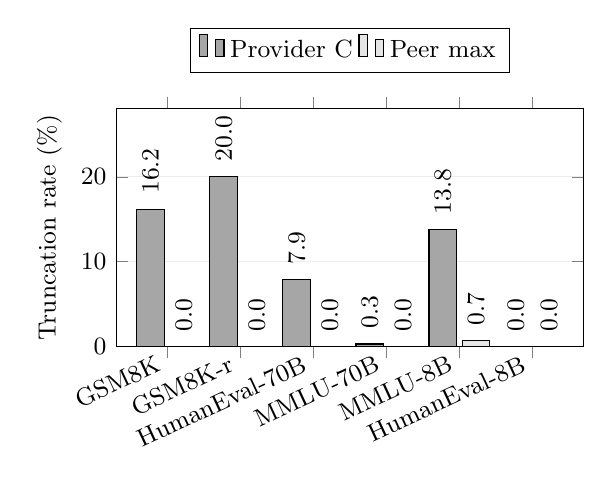
\begin{tikzpicture}
\begin{axis}[
  ybar, bar width=10pt,
  width=0.62\textwidth, height=4.6cm,
  ylabel={Truncation rate (\%)},
  symbolic x coords={GSM8K,GSM8K-r,HumanEval-70B,MMLU-70B,MMLU-8B,HumanEval-8B},
  xtick=data,
  x tick label style={font=\small, rotate=25, anchor=east},
  ylabel style={font=\small},
  yticklabel style={font=\small},
  ymin=0, ymax=28,
  ymajorgrids, grid style={gray!15, thin},
  enlarge x limits=0.14,
  legend style={font=\small, at={(0.5,1.15)}, anchor=south, legend columns=2},
  nodes near coords style={font=\small, anchor=west, rotate=90,
    xshift=2pt, /pgf/number format/fixed,
    /pgf/number format/precision=1, /pgf/number format/fixed zerofill},
]
\addplot[fill=gray!70, nodes near coords] coordinates {
  (GSM8K,16.2) (GSM8K-r,20.0) (HumanEval-70B,7.9)
  (MMLU-70B,0.3) (MMLU-8B,13.8) (HumanEval-8B,0.0)
};
\addplot[fill=gray!20, nodes near coords] coordinates {
  (GSM8K,0.0) (GSM8K-r,0.0) (HumanEval-70B,0.0)
  (MMLU-70B,0.0) (MMLU-8B,0.7) (HumanEval-8B,0.0)
};
\legend{Provider~C, Peer max}
\end{axis}
\end{tikzpicture}
\caption{Provider~C's truncation rate against the maximum rate
observed for any peer provider, per cell. GSM8K-r is the independent
100-item resample from the breadth sweep (Section~\ref{sec:breadth}).
Peer-max values are at or below 0.7\% in every cell; exact figures are
also in Table~\ref{tab:anchor}.}
\label{fig:anchor_chart}
\end{figure*}

Provider~C's failure mode depends on which model is being served. On
the 70B model, truncations are overt: the API itself reports an error
and no answer is returned. On the 8B model, the one clean-completion
generation observed after applying our audit protocol (\ref{sec:audit}
below) still leaves a genuine silent-failure rate that is absent from
every other provider serving the same model. The same underlying
provider therefore fails honestly on one model and dishonestly on
another, which we return to in Section~\ref{sec:finish_reason}.

We considered and reject an explanation based on output length.
Across the five cells in Table~\ref{tab:anchor}, truncation rate does
not track average completion length: HumanEval on the 70B model
produces longer completions on average (415 tokens) than GSM8K (154
tokens) but shows a lower truncation rate (7.9\% versus 16.2\%), and
MMLU on the 70B model produces the shortest completions of any cell
(2 tokens) and is also the cleanest. A cross-cell correlation between
average output length and Provider~C's truncation rate is weak and in
the wrong direction to explain the pattern (Spearman
$\rho{=}{-}0.10$).

\subsection{The Pathology Is Deterministic and Item-Specific}
\label{sec:determinism}

If Provider~C's truncations were caused by transient infrastructure
noise, such as momentary load spikes or rate-limit contention, we
would expect them to be roughly randomly distributed across the 300
GSM8K items and across the 3 repeated trials of each item at
temperature 0. Under an independent-failure null model, each of the 3
repeated calls for a given item truncates with probability equal to
the observed base rate $p = 0.162$, independently of the other two
calls and of the item itself. The expected number of items with
exactly $k$ truncated repeats out of 3, over $N = 300$ items, is then

\[
E[k] = N \binom{3}{k} p^k (1-p)^{3-k}.
\]

Table~\ref{tab:item} compares this expectation against the observed
distribution.

\begin{table}[t]
\centering
\small
\begin{tabular}{lrr}
\toprule
\textbf{Truncations / item (of 3)} & \textbf{Observed} & \textbf{Expected} \\
\midrule
0 & 232 & 176 \\
1 & 21  & 102 \\
2 & 16  & 20  \\
3 & 31  & 1   \\
\bottomrule
\end{tabular}
\caption{Distribution of GSM8K items by number of repeated trials (of
3) on which Provider~C truncated, observed versus the count expected
under an independent per-call failure model at the observed 16.2\%
base rate.}
\label{tab:item}
\end{table}

Thirty-one items truncate on all three repeated trials, against fewer
than one expected under a random-failure model, while the
one-truncation-of-three bucket is far below what randomness predicts.
At temperature 0, the same input reliably produces the same failure on
this provider. This is evidence of a content-triggered, reproducible
defect rather than stochastic serving noise, and it is, to our
knowledge, the most specific characterization available of what kind
of failure this is, even without access to the underlying serving
infrastructure to identify its root cause.

\subsection{A Failure Consistency Coefficient}
\label{sec:icc}

The binomial comparison above is specific to GSM8K and to a single
repeat count. To quantify item-level determinism in a form that
generalizes across benchmarks and is directly comparable to any
provider or condition, we borrow a standard measurement-theory tool.
For a given provider on a given benchmark, we treat each item as a
subject and each of its $k{=}3$ repeated trials as a replicate
measurement of a binary outcome (truncated or not), and compute the
one-way random-effects intraclass correlation coefficient,

\[
\mathrm{ICC}(1,1) = \frac{\mathrm{MS}_B - \mathrm{MS}_W}
{\mathrm{MS}_B + (k-1)\,\mathrm{MS}_W},
\]

\noindent where $\mathrm{MS}_B$ and $\mathrm{MS}_W$ are the between-item
and within-item mean squares from a one-way ANOVA on the truncation
indicator. ICC(1,1) is the fraction of total outcome variance
attributable to differences between items rather than to
repeat-to-repeat noise within an item; a value near~0 indicates
failures are effectively random with respect to item identity, and a
value near~1 indicates failures are almost entirely determined by
which item is being processed. We refer to this quantity as a
\textbf{Failure Consistency Coefficient (FCC)} when applied to
provider truncation behavior, and report 95\% confidence intervals via
item-level bootstrap (10,000 resamples).

\begin{table}[t]
\centering
\small
\begin{tabular}{lrr}
\toprule
\textbf{Cell} & \textbf{Provider~C FCC} & \textbf{Peer FCC} \\
\midrule
GSM8K / 70B      & 0.698 [0.604, 0.783] & undefined \\
HumanEval / 70B  & 0.751 [0.550, 0.887] & undefined \\
MMLU / 8B        & 0.935 [0.881, 0.979] & undefined \\
\bottomrule
\end{tabular}
\caption{Failure Consistency Coefficient (ICC(1,1), 95\% bootstrap CI)
for Provider~C's truncation outcome, by cell. Peer providers (Nebius
on GSM8K, AkashML on HumanEval, DeepInfra on MMLU/8B) show zero
truncations and thus zero outcome variance; the FCC is mathematically
undefined (0/0) rather than a spurious value, which is itself the
correct discriminant result: the coefficient cannot manufacture a
consistency pattern where no failures occur.}
\label{tab:fcc}
\end{table}

Table~\ref{tab:fcc} reports the FCC for Provider~C on the three cells
with enough truncations to support a stable estimate. All three
confidence intervals exclude 0 and sit in a high range (0.70--0.94),
confirming with a standard reliability statistic what
Section~\ref{sec:determinism} showed for GSM8K alone: truncation is
substantially an item property, not a repeat-to-repeat coin flip.
The three cells also differ in an interpretable way. MMLU on the 8B
model has the highest FCC (0.935): these are cap-hit failures where
the same difficult items consistently exceed the token budget without
producing a parseable letter, an almost fully deterministic pattern.
GSM8K's FCC is lower (0.698), consistent with
Section~\ref{sec:determinism}'s observation that some items truncate
on only one or two of three trials rather than all-or-nothing,
indicating a real but noisier item effect layered on top of some
residual stochasticity. HumanEval's estimate has the widest interval
(rests on 39 truncation events over 164 items) but still comfortably
excludes 0.

\subsection{\texttt{finish\_reason} Is Not a Reliable Completeness
Signal}
\label{sec:finish_reason}

Two pieces of evidence in our data show that neither a provider's own
self-reported completion status, nor a naive automated completeness
check, can be trusted without verifying the actual generated text.

First, on the MMLU cell for the 8B model, Provider~C reports
\texttt{finish\_reason=stop} on the incomplete generations counted in
Table~\ref{tab:anchor}, while every peer provider that reaches the
same token budget on the same benchmark correctly reports
\texttt{finish\_reason=length}. Provider~C's self-report is
inconsistent with what actually happened.

\subsubsection{Audit protocol in practice}
\label{sec:audit}

Second, we flagged four candidate silent failures on the 8B model
during a broader provider survey (Section~\ref{sec:breadth}), on two
providers other than Provider~C. On manual inspection of the raw
completion text, all four were complete, correct answers: each ended
with a phrase such as ``The final answer is: \$X'' rather than the
expected delimiter, giving the correct numeric answer in full. None
was actually truncated. Table~\ref{tab:audit} lists all four cases.

\begin{table}[t]
\centering
\footnotesize
\begin{tabular}{lrrc}
\toprule
\textbf{Provider} & \textbf{Tokens} & \textbf{Answer} & \textbf{Verdict} \\
\midrule
Novita  & 216 & correct & complete \\
WandB   & 163 & correct & complete \\
WandB   & 180 & correct & complete \\
WandB   & 259 & correct & complete \\
\bottomrule
\end{tabular}
\caption{All four candidate silent-failure flags raised during the
breadth survey (Section~\ref{sec:breadth}), audited against the raw
completion. Token counts are well under the 1024-token budget in every
case, and every completion ends with a stated numeric answer matching
the gold answer; none is truncated.}
\label{tab:audit}
\end{table}

We had encountered the identical failure mode once before, during a
smaller pilot run, and had already corrected our audit protocol to
catch it; the fact that it recurred at full scale on a different
provider pair confirms that this is a systematic property of how the
8B model closes its answers, not a one-off annotation error, and that
automated completeness flags on this model require verification
before being reported as findings. We report both the automated flag
rate and the audited, corrected rate throughout this paper, and every
reliability number in Table~\ref{tab:anchor} is the audited figure.

\subsection{Breadth: Is This Provider-Specific?}
\label{sec:breadth}

To test whether the truncation pathology in Section~\ref{sec:reliability}
is unique to Provider~C or a more general property of the provider
marketplace, we ran an independent breadth sweep across all 26
canonical provider deployments spanning the 6 models surveyed in
Table~\ref{tab:models}, using GSM8K at 100 items per deployment.
Table~\ref{tab:breadth} summarizes the outcome by model. After
applying the audit protocol from Section~\ref{sec:audit} to every
automatically flagged candidate, Provider~C remains the only confirmed
truncator across all 26 deployments. This breadth check is what
independently reproduces the 20\% GSM8K rate reported in
Table~\ref{tab:anchor}, on a disjoint sample collected separately from
our main GSM8K run.

\begin{table}[t]
\centering
\small
\begin{tabular}{lrrr}
\toprule
\textbf{Model} & \textbf{Providers} & \textbf{Raw flags} & \textbf{Confirmed} \\
\midrule
Llama-3.3-70B & 11 & 1 & 1 (Provider~C) \\
Llama-3.1-70B & 3  & 0 & 0 \\
Llama-3.1-8B  & 6  & 2 & 0 \\
Qwen-2.5-72B  & 1  & 0 & 0 \\
Qwen-2.5-7B   & 2  & 0 & 0 \\
Gemma-2-27B   & 1  & 0 & 0 \\
\midrule
Total         & 24 & 3 & 1 \\
\bottomrule
\end{tabular}
\caption{Breadth sweep outcome by model, GSM8K, 100 items per
deployment. ``Raw flags'' counts deployment-provider pairs with at
least one automated silent-failure flag; ``Confirmed'' counts those
that survive manual audit against the raw completion. Provider~C's
count on Llama-3.3-70B is its already-established overt-failure
pathology; the two raw flags on Llama-3.1-8B are the audited false
positives in Table~\ref{tab:audit}.}
\label{tab:breadth}
\end{table}

%-------------------------------------------------------------------
\section{Discussion}

\subsection{A Reporting Checklist}

Our results argue for treating provider identity as a first-class
variable in any API-based LLM evaluation, alongside model name,
prompt, and decoding parameters. Table~\ref{tab:checklist} lists the
fields we recommend every API-based evaluation report state
explicitly. Given our finding in Section~\ref{sec:determinism}, we
further recommend that studies relying on temperature-zero,
single-trial evaluation consider at least a small number of repeated
trials per item specifically to distinguish a stochastic serving
glitch from a deterministic, reproducible provider defect, since the
two have different implications for whether the failure will recur.

\begin{mdframed}[linewidth=0.5pt, linecolor=gray!50,
  innerleftmargin=6pt, innerrightmargin=6pt, innertopmargin=3pt,
  innerbottommargin=3pt, backgroundcolor=gray!4]
\small
\textbf{Reporting checklist for API-based LLM evaluation}
\begin{itemize}[leftmargin=*, itemsep=1pt, topsep=2pt]
\item \textbf{Model identifier}, exact, including version tag.
\item \textbf{Provider identifier}, the specific serving endpoint
  used, not just the aggregator.
\item \textbf{Disclosed quantization}, if the provider reports one;
  note explicitly if undisclosed.
\item \textbf{Snapshot date} of data collection; provider identity,
  pricing, and availability all drift over time.
\item \textbf{Fallback routing policy}, whether requests could be
  silently rerouted to a different provider than requested.
\item \textbf{Repeats per item}, especially for temperature-zero
  evaluation, to separate stochastic noise from deterministic,
  reproducible failures (Section~\ref{sec:determinism}).
\end{itemize}
\end{mdframed}
\label{tab:checklist}

\subsection{On the Single-Provider Finding}

The central reliability finding in this paper concerns one provider.
We do not read this as a weakness to be argued around but as the
honest output of a broad, audited search: our contribution is not
Provider~C specifically but the measurement protocol and audit
discipline that found it, confirmed it under independent replication,
ruled out the most obvious alternative explanation, and searched 25
other deployments without finding a second instance. Whether other
providers exhibit comparable pathologies under different models,
benchmarks, or conditions is an open question our method is built to
answer, not one we claim to have closed.

%-------------------------------------------------------------------
\section{Conclusion}

Clean-completion accuracy for the models and benchmarks we test is
provider-invariant: no provider pair separates under our
pre-registered threshold, on GSM8K, MMLU, or HumanEval. Reliability is
not. One provider shows a real, replicated, content-triggered
truncation pathology that is invisible to a harness which does not
separate correctness from completeness, and would be systematically
misgraded as an accuracy deficit by one that does not audit its own
failure detector. The pathology is deterministic at the item level,
not explained by output length, and confirmed independently on both a
900-call primary run and a disjoint 100-item resample. A breadth
search across 26 deployments and six models found no second instance,
which we report as evidence of the method's reach rather than as a
closed question. Provider identity, disclosed precision, snapshot
date, and repeat count are not incidental details of an API-based
evaluation; our results show they can be the difference between a
real finding and an artifact.

%-------------------------------------------------------------------
\section{Limitations}

Our central reliability claim rests primarily on one provider; while
we conducted a 26-deployment breadth search across six models
specifically to test generality, and independently replicated the
core GSM8K result, the finding remains anchored to a single instance
rather than a class of providers. We evaluate two models, selected
because they were the only candidates among eight surveyed with
sufficient live provider coverage for this kind of study; this is
itself a finding about the current state of the provider marketplace,
but it limits how broadly our accuracy-invariance result can be
claimed to generalize. All data was collected through a single
aggregator (OpenRouter); results may not transfer to other routing
marketplaces. Our data is snapshot-dated: provider availability,
disclosed quantization, and serving behavior all changed during data
collection, including one provider that became entirely unavailable
and one that experienced a transient multi-hour outage, both handled
by exclusion and documentation rather than by treating them as part of
the reliability finding. We identify that Provider~C's truncation
pathology is deterministic and item-specific, but we do not have
access to the underlying serving infrastructure and cannot identify
its root cause, whether that is a batching policy, a timeout
configuration, or something else. Finally, our audit protocol is
manual and does not scale to arbitrarily large studies; we view this
as a genuine cost of the rigor we argue for, not an incidental
limitation.

%-------------------------------------------------------------------
\section*{Ethics Statement}

This work evaluates publicly available commercial API services using
their standard, documented interfaces and normal usage patterns; we
did not attempt to circumvent rate limits, terms of service, or access
controls. We anonymize the specific provider exhibiting the reliability
failure described in this paper for the review version of this
submission; we intend to name it directly in any final published
version, since the purpose of this work is to inform practitioners and
the affected provider of a real, verifiable, and reproducible issue
with their service, not to conceal it. All benchmarks used are public
and widely used research artifacts. We release our harness, frozen
item sets, and checksummed raw logs at
\url{https://anonymous.4open.science/r/provider-variance-eval-C614/README.md}
to support independent verification of every claim in this paper.

%-------------------------------------------------------------------
\bibliography{references}

\end{document}
